\section{SAMPLE TEXT WITH GRAPHICS} \label{graphics}
%This file illustrates how include in your thesis graphical
 %output.
%The next line produces an indented paragraph to start the document
 %unit.  The LaTeX defaults start most units without indentations.
\hspace{\parindent}
This is sample text with graphics.
\begin{figure}[h]
  \centering
  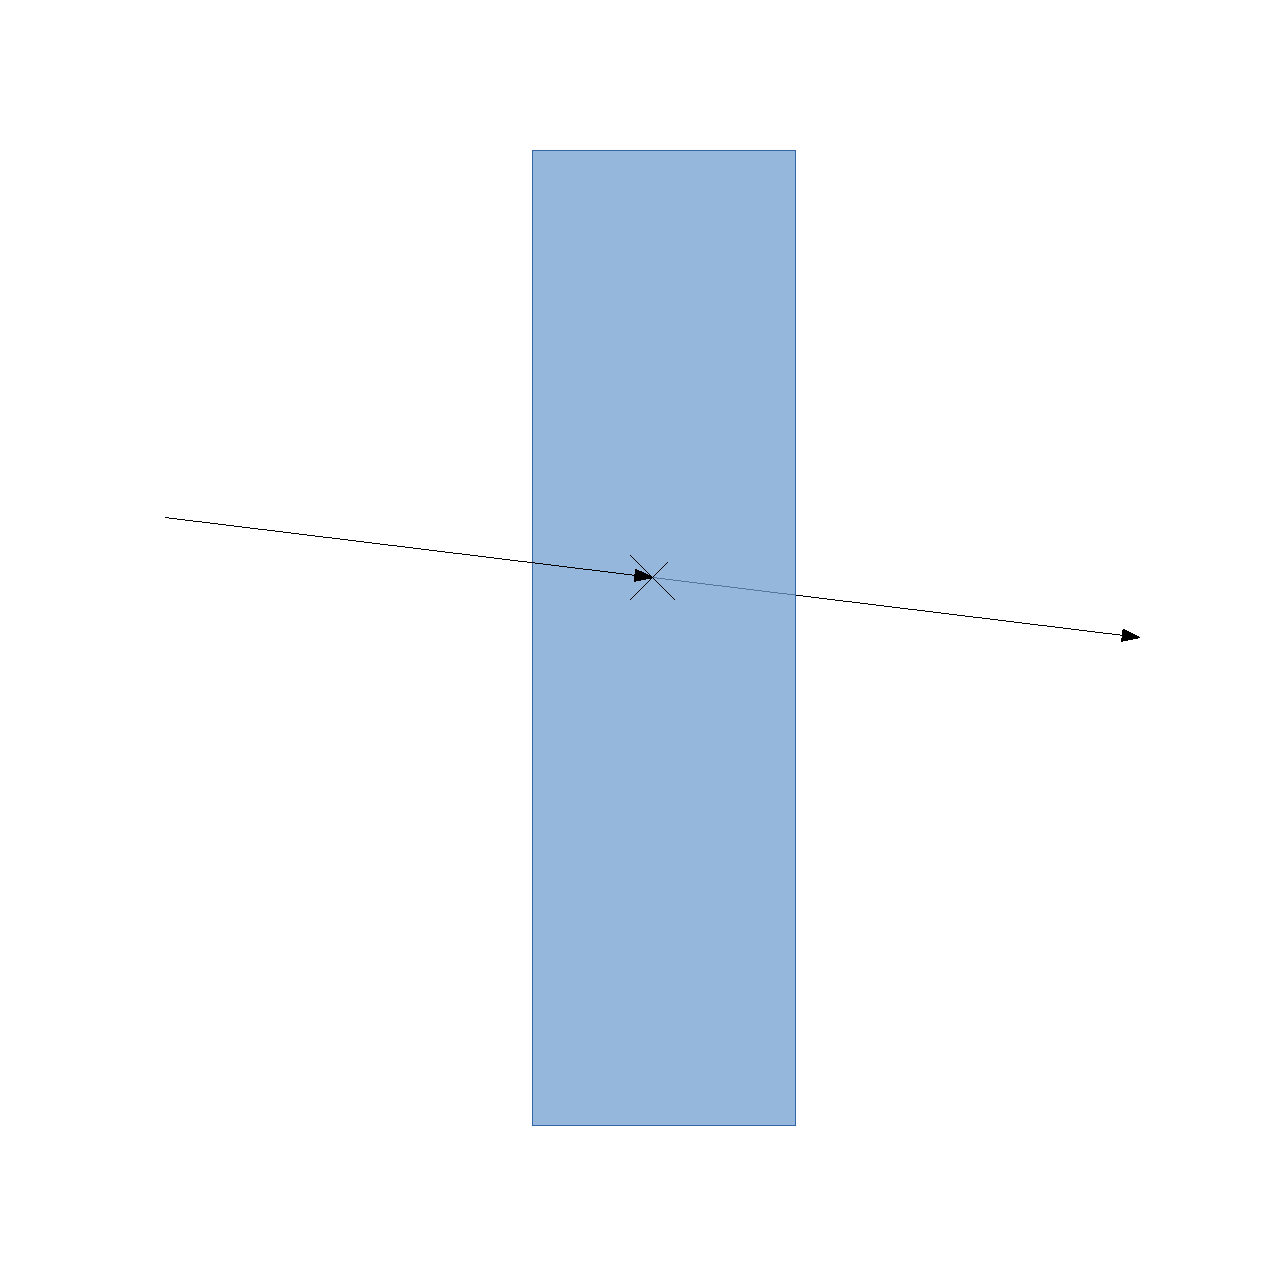
\includegraphics[angle=-90,width=4in]{figures/bz.pdf}
  \caption{This is an inserted EPS graphic}
  \label{fig:mygraph1}
\end{figure}
Sample ref of \ref{fig:mygraph1} 

\begin{figure}[t]
 \centering
  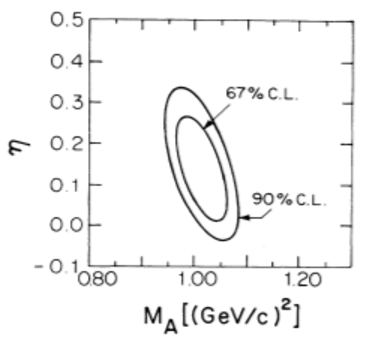
\includegraphics[angle=-90, width=4in]{figures/E734eta.pdf}  
    \caption{This is another inserted PDF graphic}
    \label{fig:mygraph2}
\end{figure}
%This is the end of the file graphics.tex

